\documentclass{article}
\usepackage{graphicx}
\usepackage{amsmath}
\usepackage{amsfonts}
\usepackage{bookmark}
\usepackage{booktabs}
\usepackage{exercises}
\graphicspath{ {./images/8.4} }
\usepackage{indentfirst}
\usepackage{amsthm}
\usepackage{yhmath}
\usepackage{geometry}
\usepackage{placeins}
\usepackage{csquotes}
\usepackage{pgfplots}
\newcommand*{\oldneg}{\mathord{\sim}}
\newcommand\showdiv[1]{\overline{\smash{)}#1}}
\newcommand\Mydiv[1]{%
\smash{\raise.3ex\hbox{$\big)$}}\mkern-8mu
        \overline{\enspace\strut#1}}
\setlength{\tabcolsep}{5pt}
\theoremstyle{definition}
\newtheorem{definition}{Definition}

\setlength{\parindent}{.5in}
\setlength{\parskip}{12pt}
\renewcommand{\arraystretch}{2}
\geometry{margin=1in}
\newcommand{\?}{\stackrel{?}{=}}
\pgfplotsset{width=7cm,compat=1.18}\usepgfplotslibrary{statistics}

\title{8.4 Answers}
\begin{document}
\maketitle

\section*{1}
An ellipse is the set of all points $P$ such that the sum of the distances between $P$ and two fixed points, called the foci, is a constant.

\section*{2}
There are two cases for the vertices and co-vertices: the vertices are $(\pm a,0)$ and the co-vertices are $(0,\pm b)$, or the vertices are 
$(0,\pm a)$ and the co-vertices are $(\pm b,0)$. In any case, we are given both the values of $a$ and $b$. It is known that $c^2=a^2-b^2$, where 
$c$ is the distance from the center of the ellipse to the foci. Thus we can then find $c$. In the first case (where the vertices are $(\pm a,0)$ and 
the co-vertices are $(0,\pm b)$) we then know that the foci are $(\pm c,0)$. In the second case, we know that the foci are $(0,\pm c)$.

\section*{4}
We are given the equation \[ \frac{x^2}{4}+y^2=25 \] \[ \frac{x^2}{100}+\frac{y^2}{25}=1 \] meaning 
$a=\sqrt{100}=10$ and $b=\sqrt{25}=5$. Thus the vertices are $(\pm 10,0)$ and the co-vertices are $(0,\pm 5)$. Then 
\[ c^2=100-25 \] \[ c=\sqrt{75} \] meaning the foci are $(\pm\sqrt{75},0)$:\newline
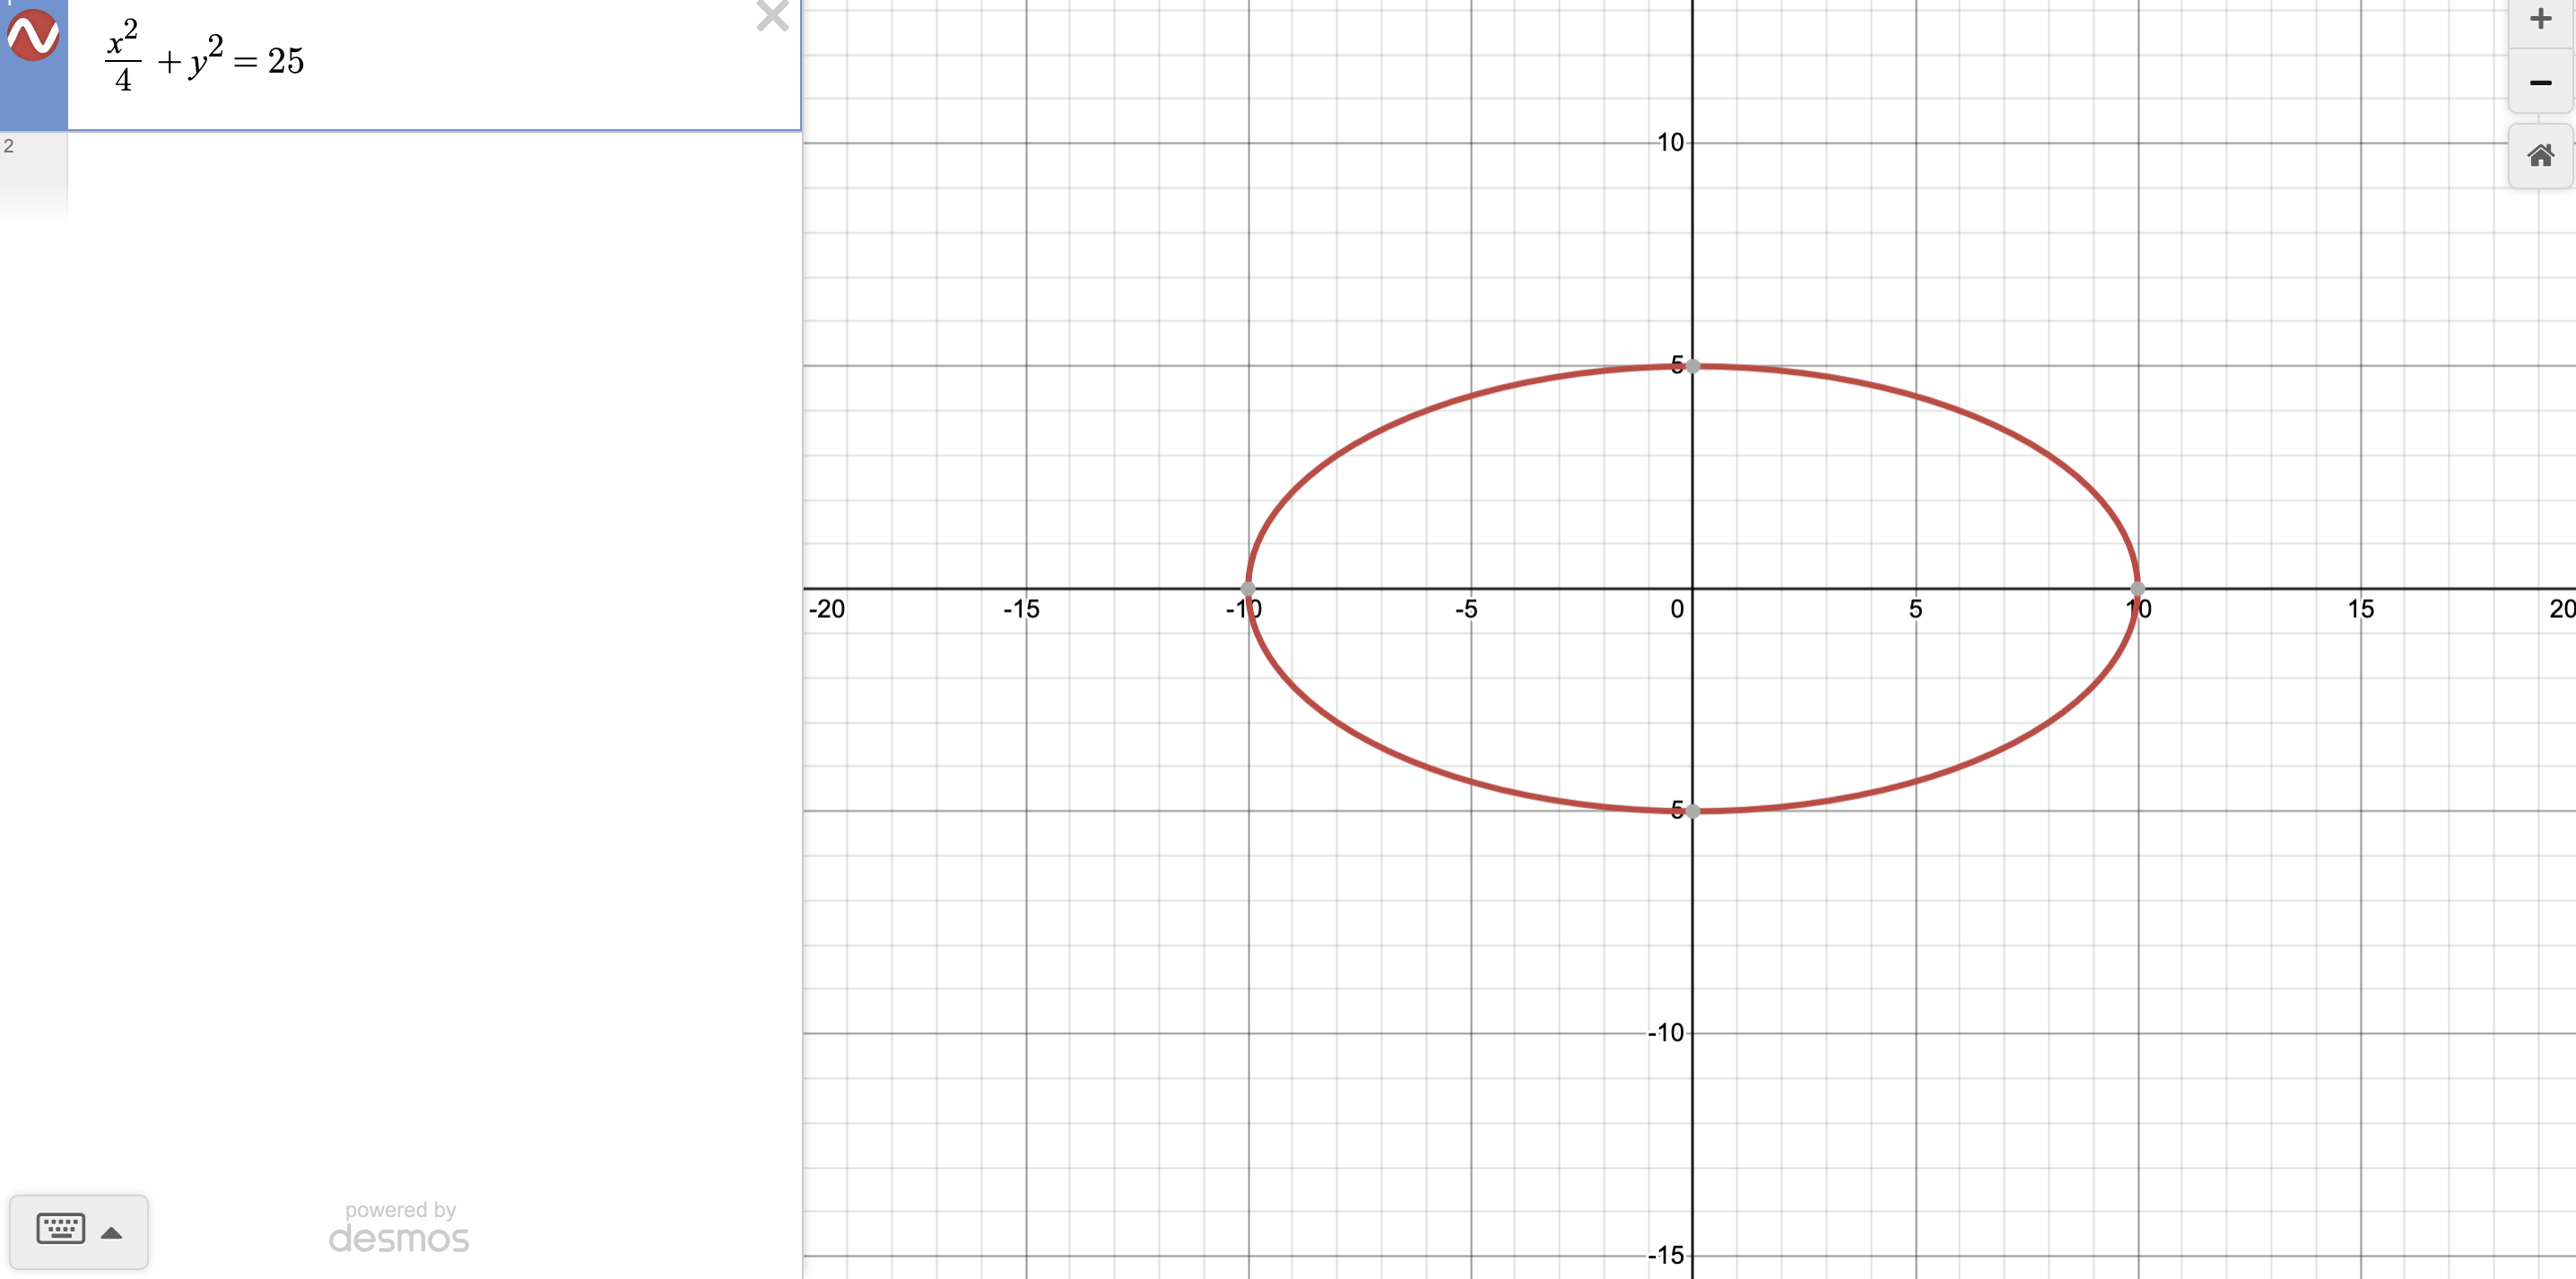
\includegraphics[width = 4in, height = 4in]{4}

\section*{7}
We know that $a=\sqrt{400}=20$ and $b=\sqrt{81}=9$. Thus the vertices are $(\pm 9, 0)$ and the co-vertices are $(0,\pm 20)$. Then 
\[ c^2=400-9 \] \[ c=\sqrt{391} \] meaning the foci are $(\pm \sqrt{391},0)$:\newline
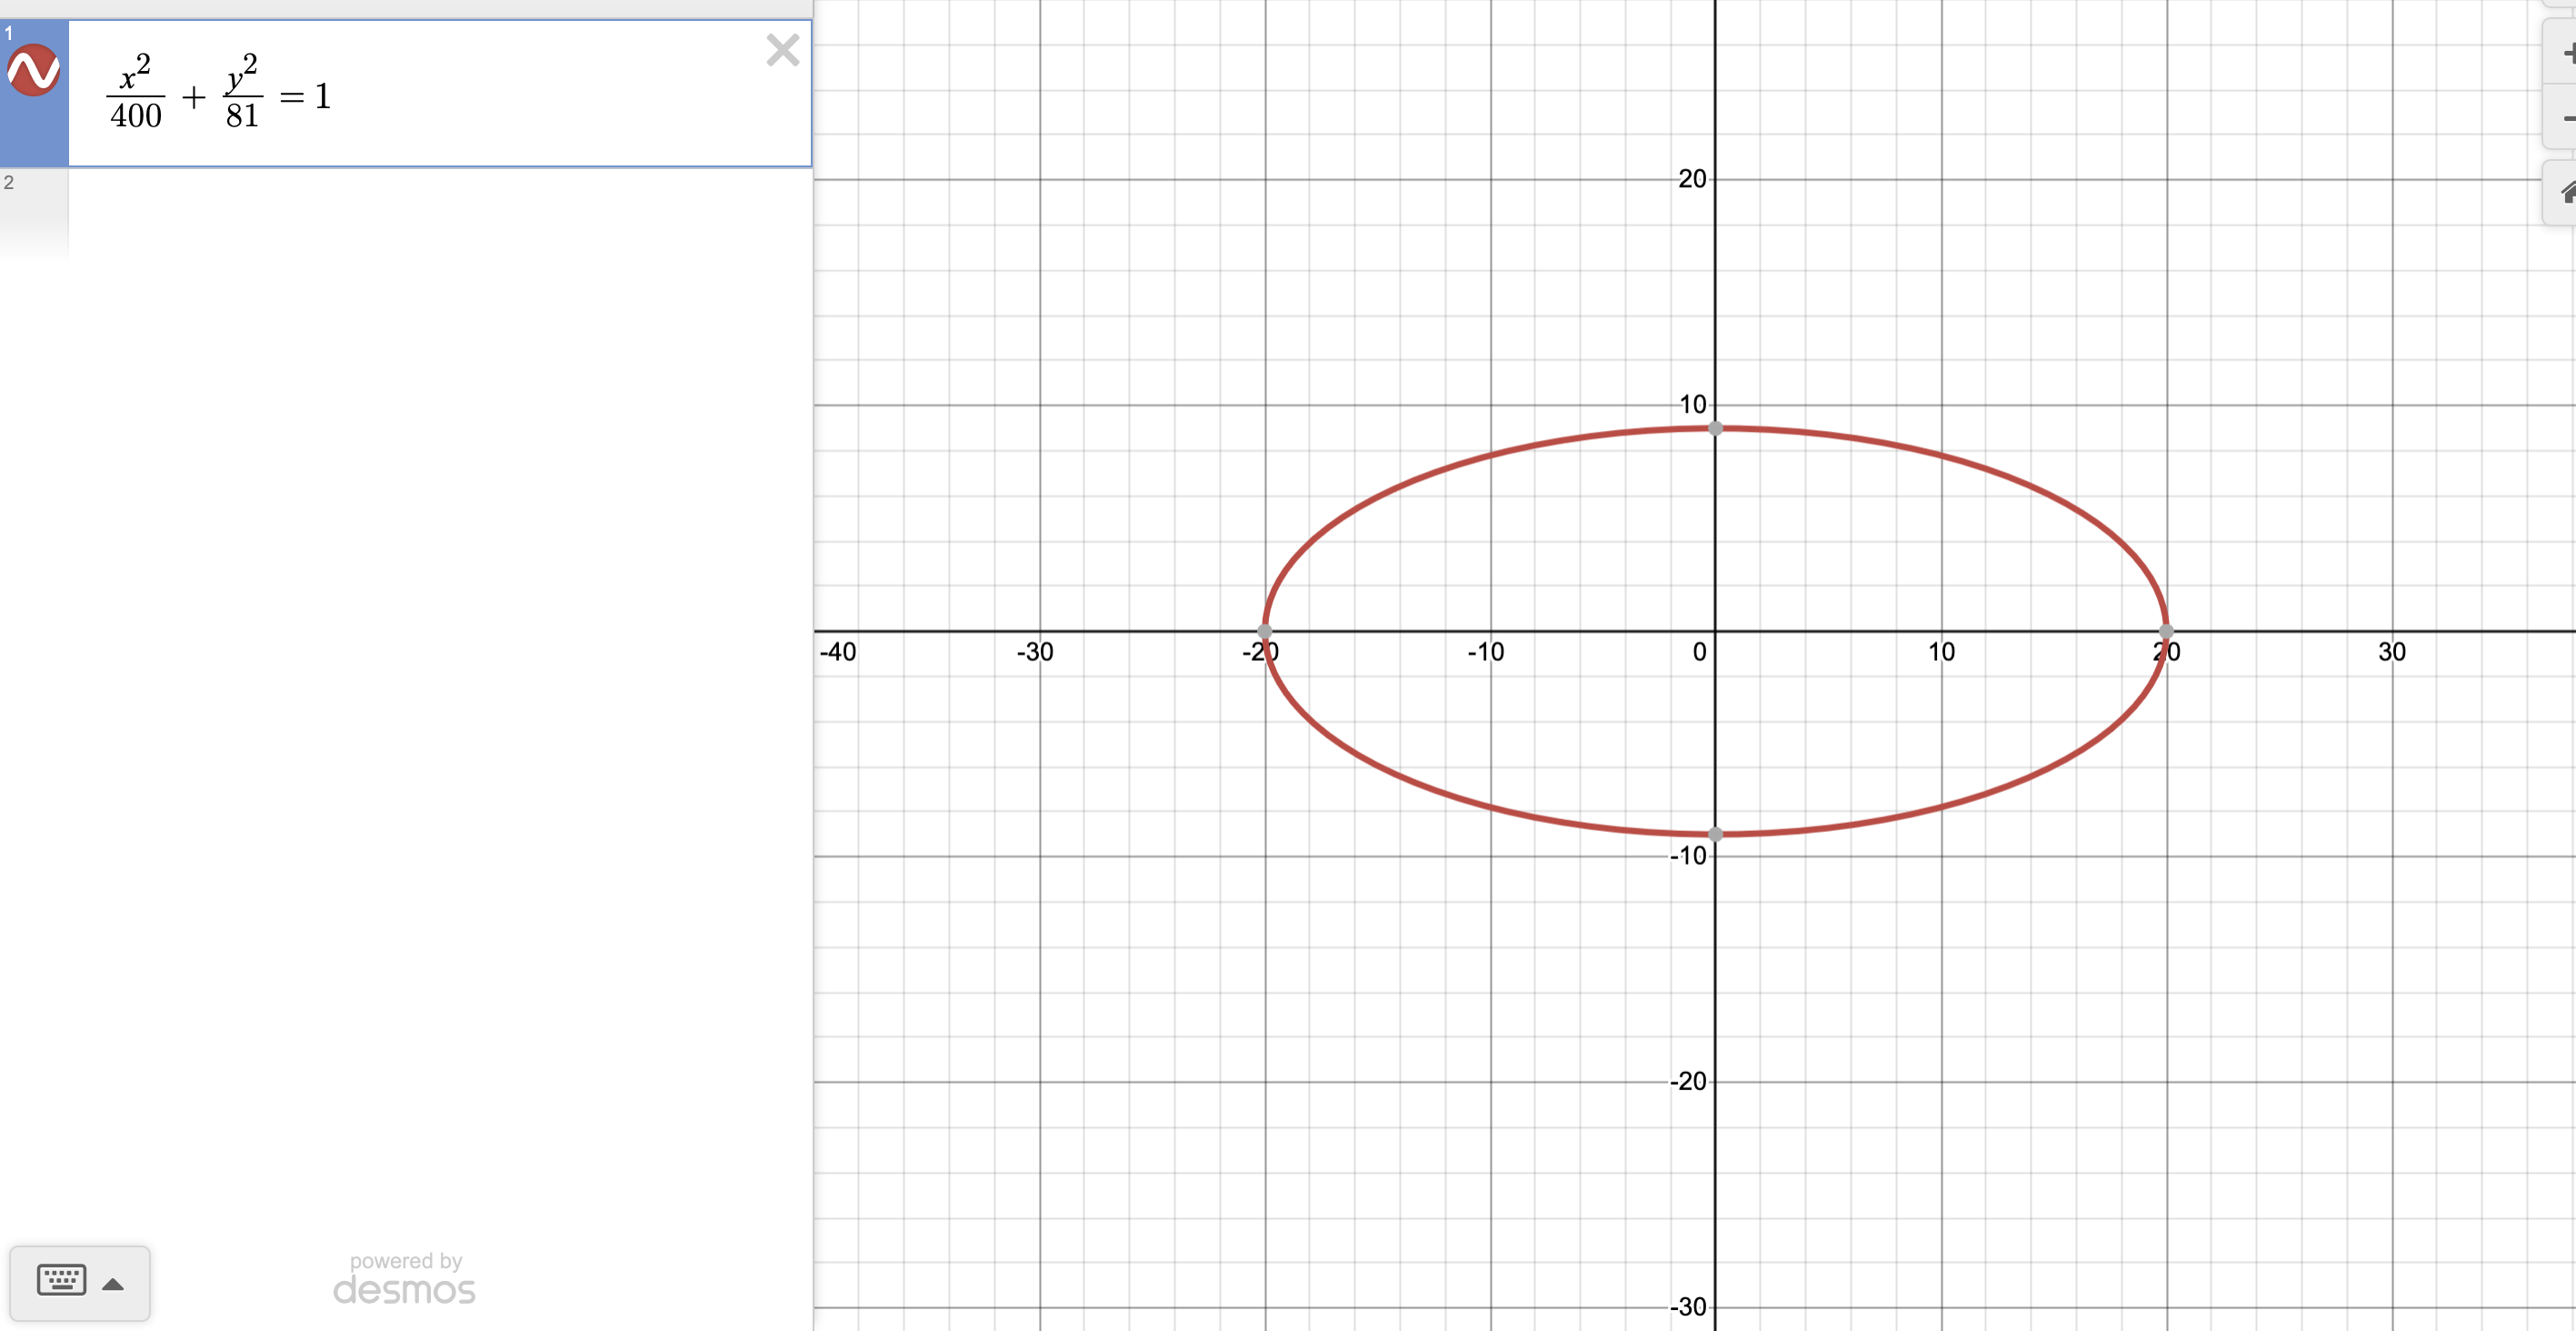
\includegraphics[width = 4in, height = 4in]{7}

\section*{11}
We are given the equation \[ 16x^2+9y^2=144 \] \[ \frac{x^2}{9}+\frac{y^2}{16}=1 \]
Then $a=\sqrt{16}=4$ and $b=\sqrt{9}=3$, meaning, because the major axis is vertical, the vertices are $(0,\pm 4)$, and the co-vertices are $(\pm 3,0)$. Then 
\[ c^2=16-9 \] \[ c=\sqrt{7} \] meaning the foci are $(0,\pm\sqrt{7})$:\newline
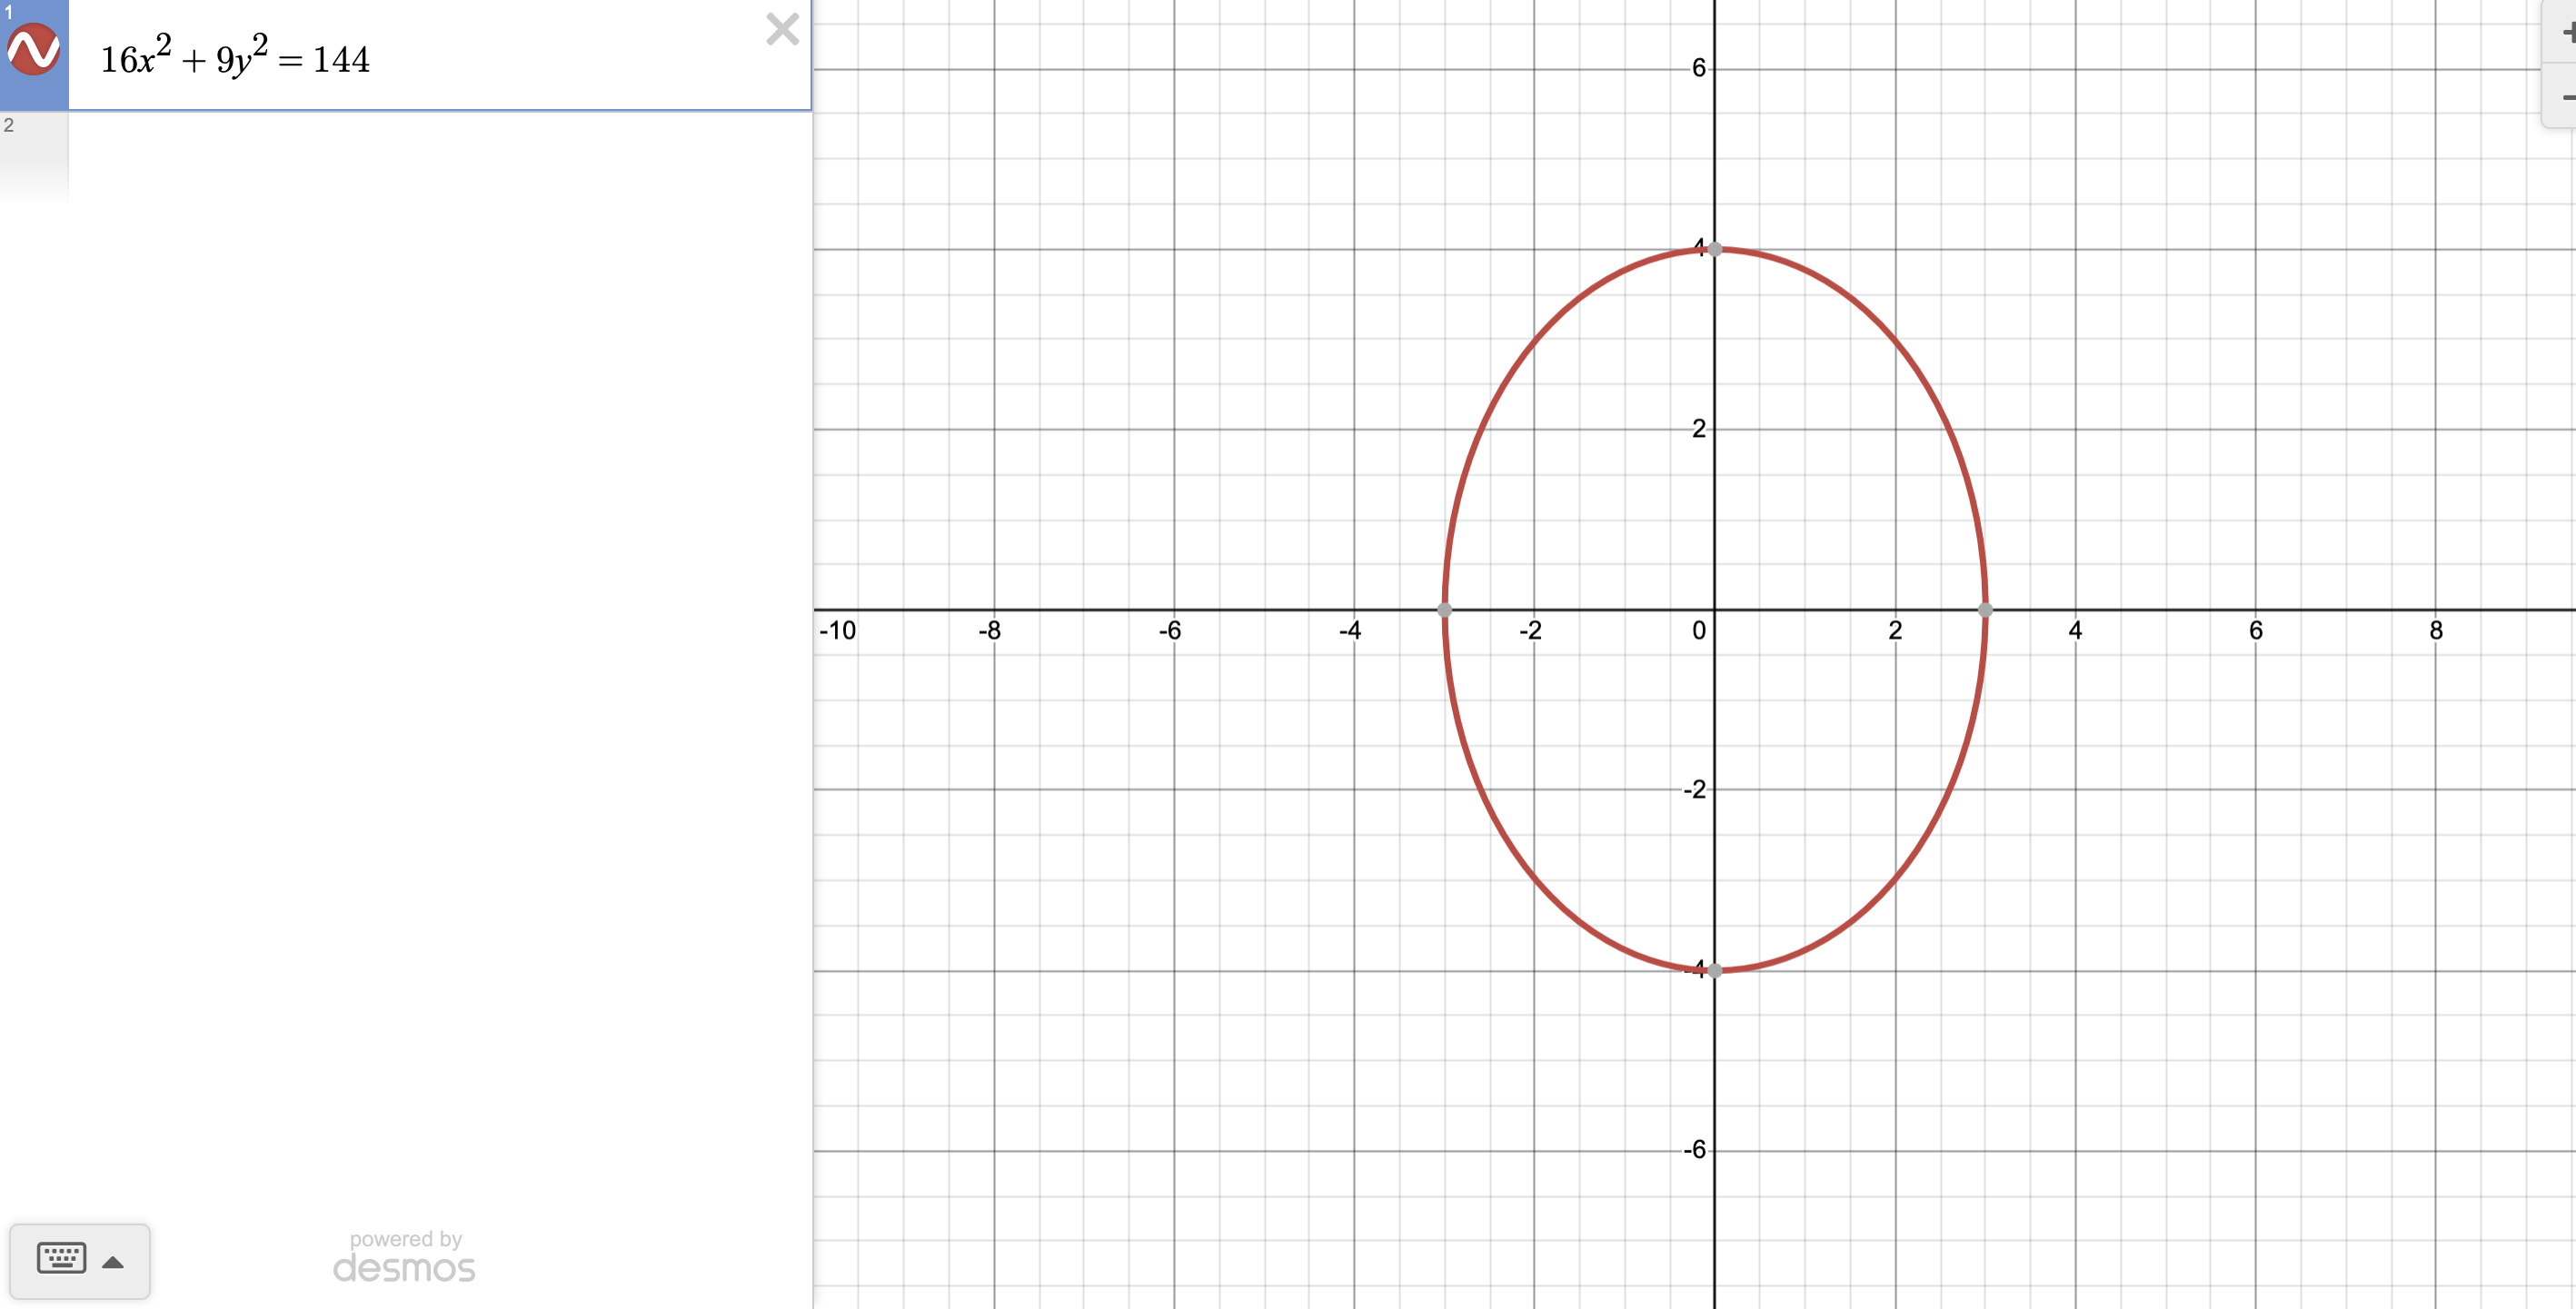
\includegraphics[width = 4in, height = 4in]{11}

\section*{21}
We are given a vertex of $(0,12)$ and a co-vertex of $(11,0)$, meaning $a=12$ and $b=11$, meaning the equation for the ellipse is (because the vertices are of the 
form $(\pm a,0)$)
$\frac{x^2}{11^2}+\frac{y^2}{12^2}=1$.

\section*{22}
We are given a vertex of $(20,0)$ and a co-vertex of $(0,-16)$, meaning $a=20$ and $b=16$, meaning 
the equation for the ellipse is $\frac{x^2}{20^2}+\frac{y^2}{16^2}=1$.

\section*{27}
We are given a vertex of $(0,-4)$ and a focus of $(\sqrt{7},0)$. Thus we know that $a=4$ and $c=\sqrt{7}$. Then we know that:
\[ (\sqrt{7})^2=4^2-b^2 \] \[ b^2=9 \] \[ b=3 \] Because the vertex is of the form $(0,-4)$, the equation for the ellipse is $\frac{x^2}{3^2}+\frac{y^2}{4^2}=1$.

\section*{28}
We are given a vertex of $(13,0)$ and a focus of $(-4\sqrt{3}, 0)$. Thus we know that $a=13$ and $c=4\sqrt{3}$. Then we know that:
\[ (4\sqrt{3})^2=13^2-b^2 \] \[ b^2=121 \] \[ b=11 \] Because the vertices are of the form $(\pm a,0)$, the equation for the ellipse is
$\frac{x^2}{13}+\frac{y^2}{11}=a$.

\section*{33}
We are given a co-vertex of $(2\sqrt{15},0)$ and a focus of $(0,14)$. Thus $b=2\sqrt{15}$ and $c=14$. Then we know that:
\[ 14^2=a^2-(2\sqrt{15})^2 \] \[ a^2=256 \] \[ a=16 \] Because the co-vertices are of the form $(\pm b, 0)$, the equation for the ellipse is
\[ \frac{x^2}{(2\sqrt{15})^2}+\frac{y^2}{16^2}=1 \]
\[ \frac{x^2}{60}+\frac{y^2}{256}=1 \]

\section*{35}
We are given a vertex of $(0,-12)$ and a co-vertex of $(-8,0)$. Thus $a=12$ and $b=8$, and because the vertices are of the form $(0,\pm a)$, the equation for the 
ellipse is $\frac{x^2}{8^2}+\frac{y^2}{12^2}=\frac{x^2}{64}+\frac{y^2}{144}=1$. B

\section*{37}
We are given the equation \[ 25x^2+81y^2=2025 \] \[ \frac{x^2}{81}+\frac{y^2}{25}=1 \] meaning this is an equation of an ellipse with 
$a=\sqrt{81}=9$ and $b=\sqrt{25}=5$. Thus the vertices are $(\pm 9,0)$ and the co-vertices are $(0,\pm 5)$ and the major axis is horizontal:\newline
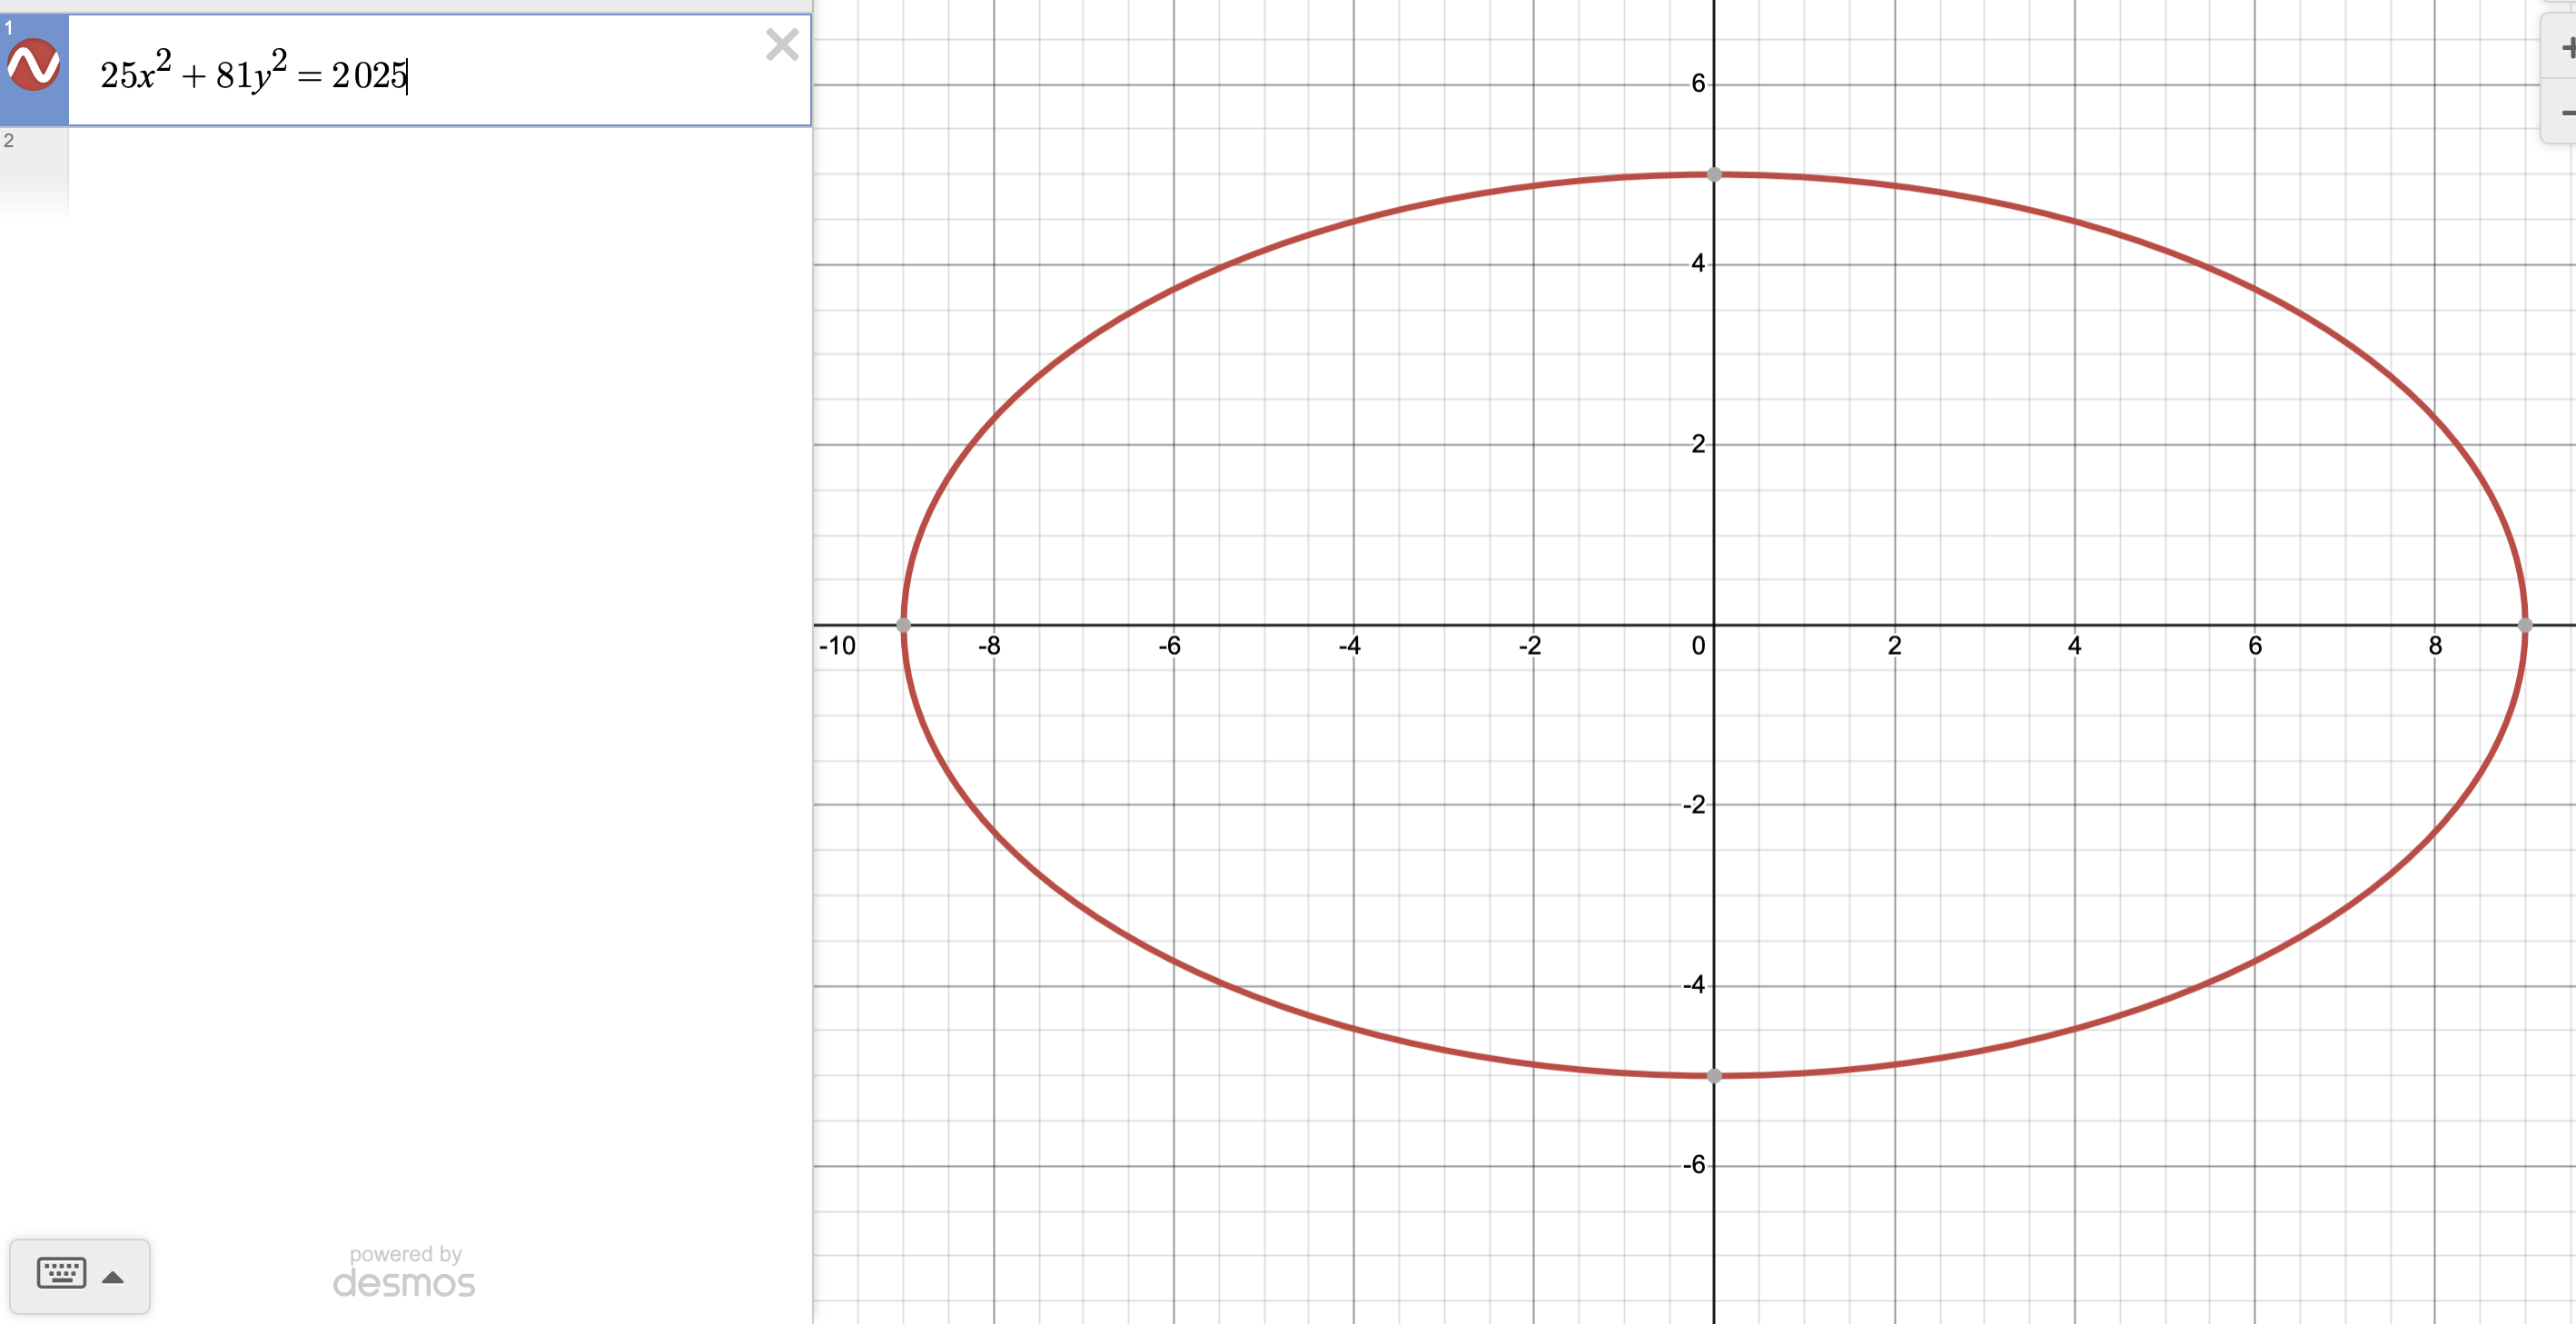
\includegraphics[width = 4in, height = 4in]{37}

\section*{39}
We are given the equation \[ 65y^2=130x \] \[ y^2=2x \] meaning this is an equation of a parabola with $p=\frac{2}{4}=\frac{1}{2}$. Thus the axis of symmetry is 
$y=0$, the focus is $(\frac{1}{2},0)$, and the directrix is $x=-\frac{1}{2}$:\newline
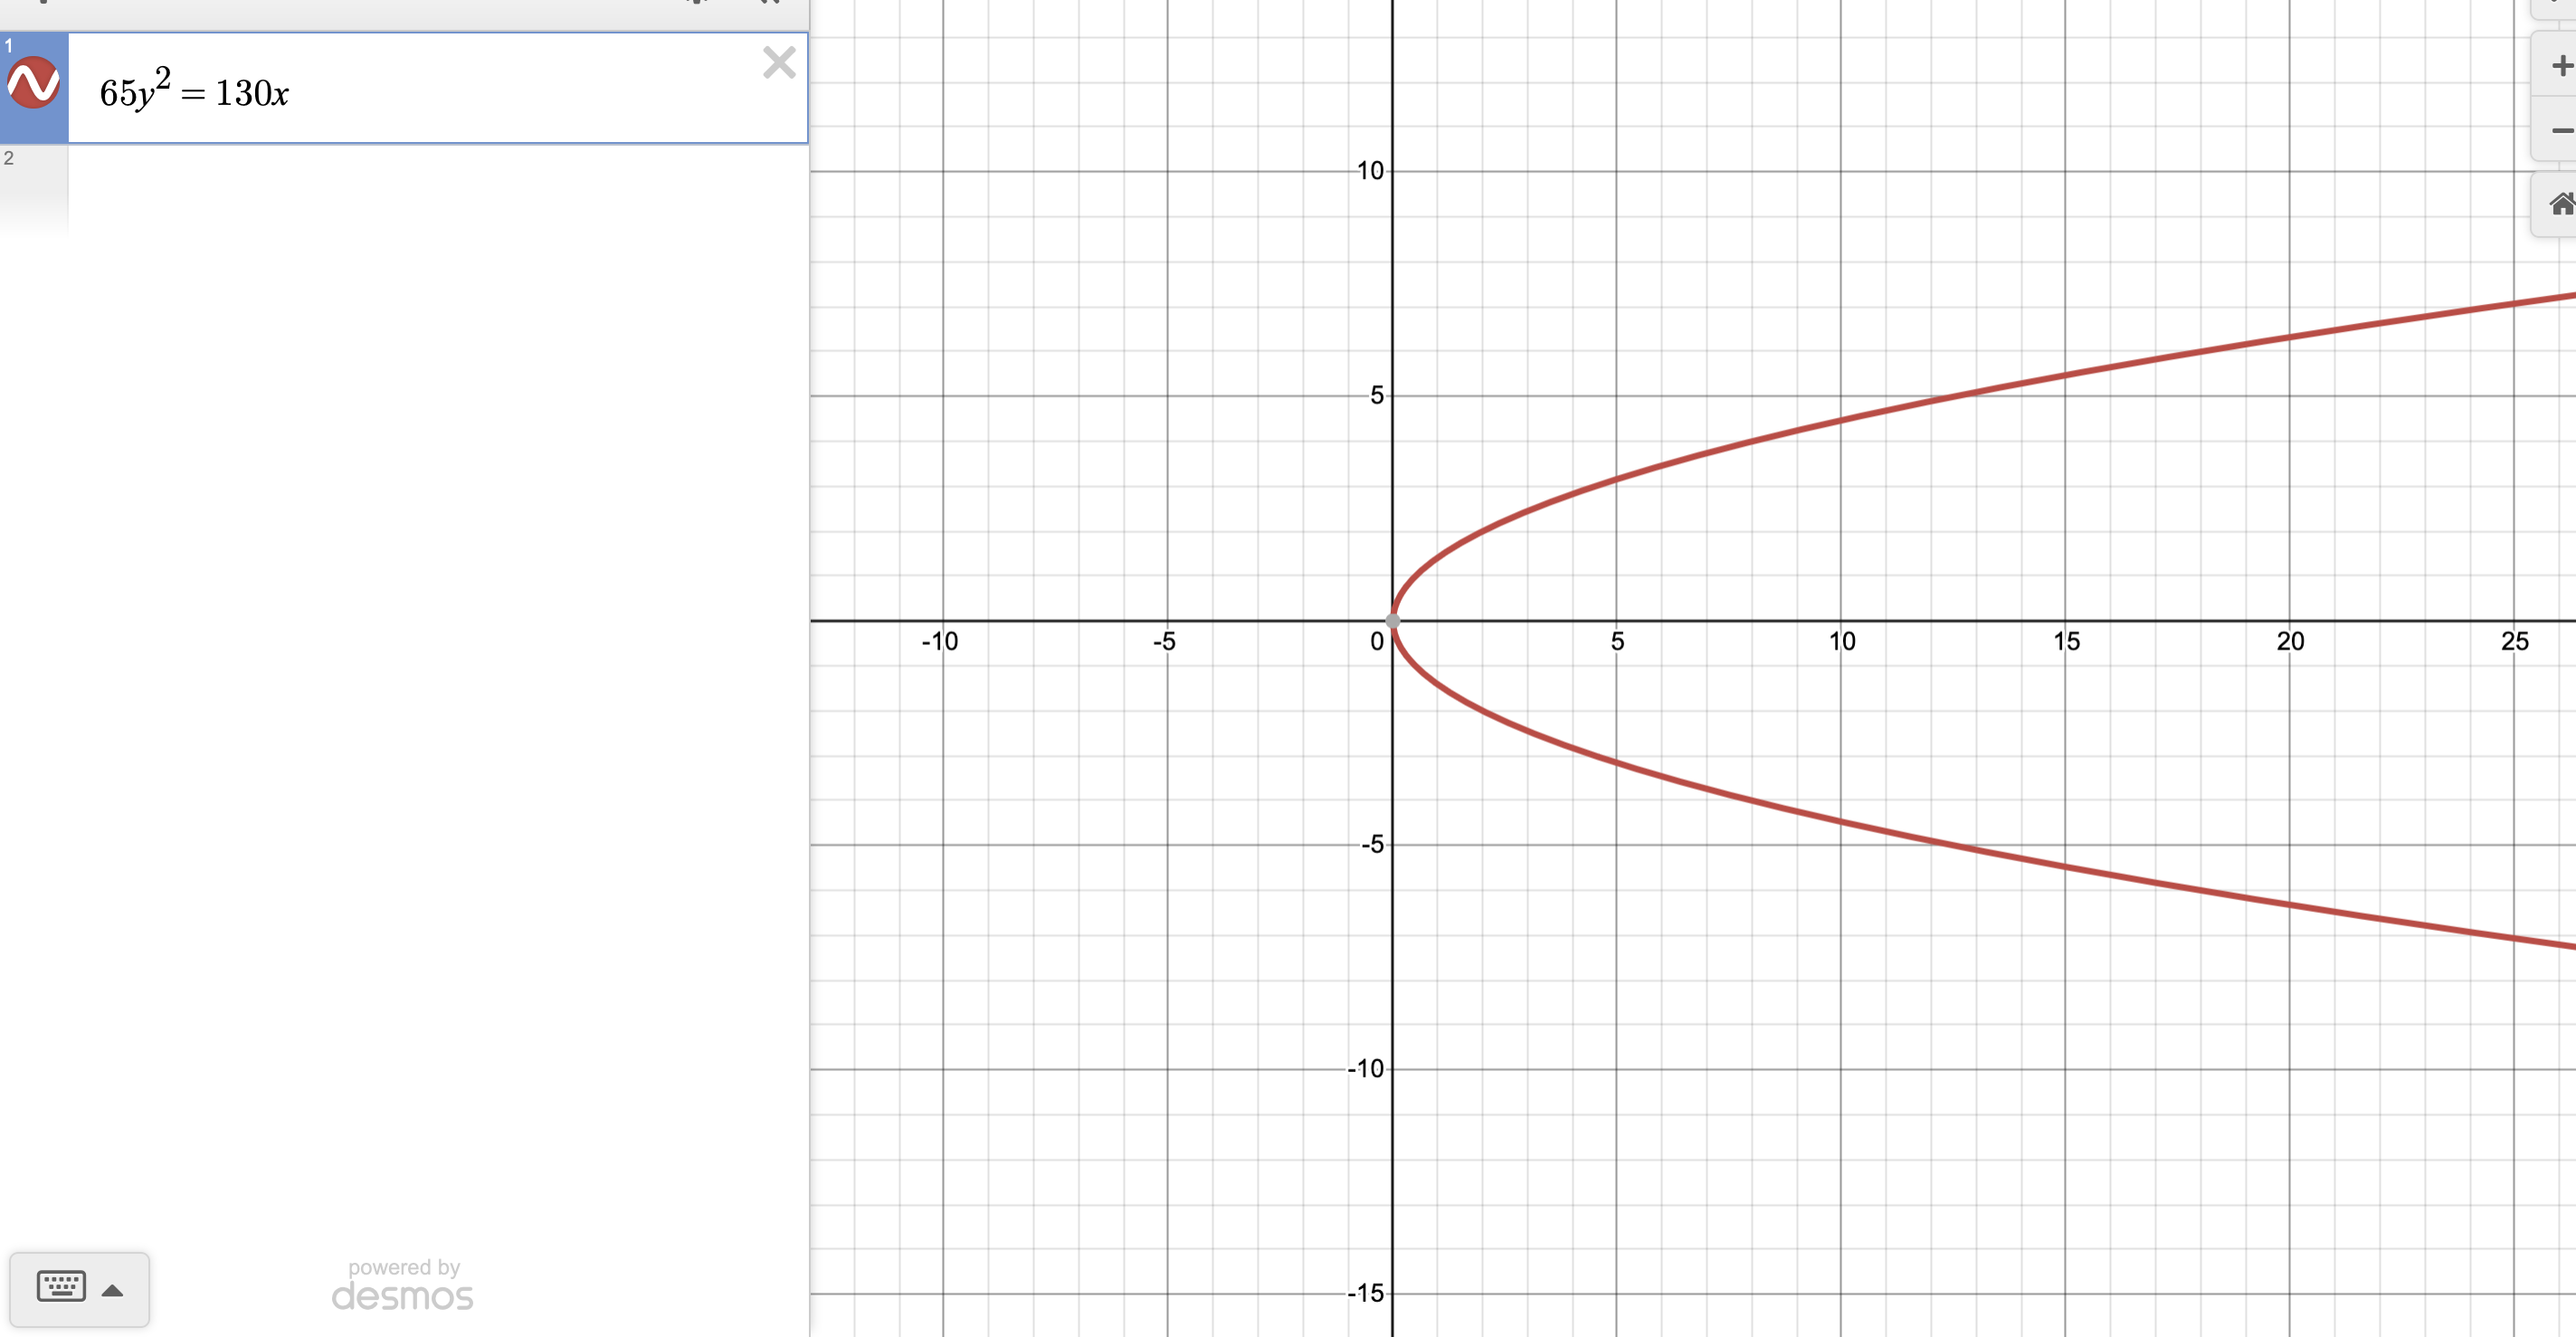
\includegraphics[width = 4in, height = 4in]{39}

\section*{43}
We are given the equation \[ \frac{x^2}{64}+\frac{y^2}{64}=4 \] \[ x^2+y^2=256 \] meaning this is an equation of a circle centered at the origin with a radius of 
$\sqrt{256}=16$:\newline
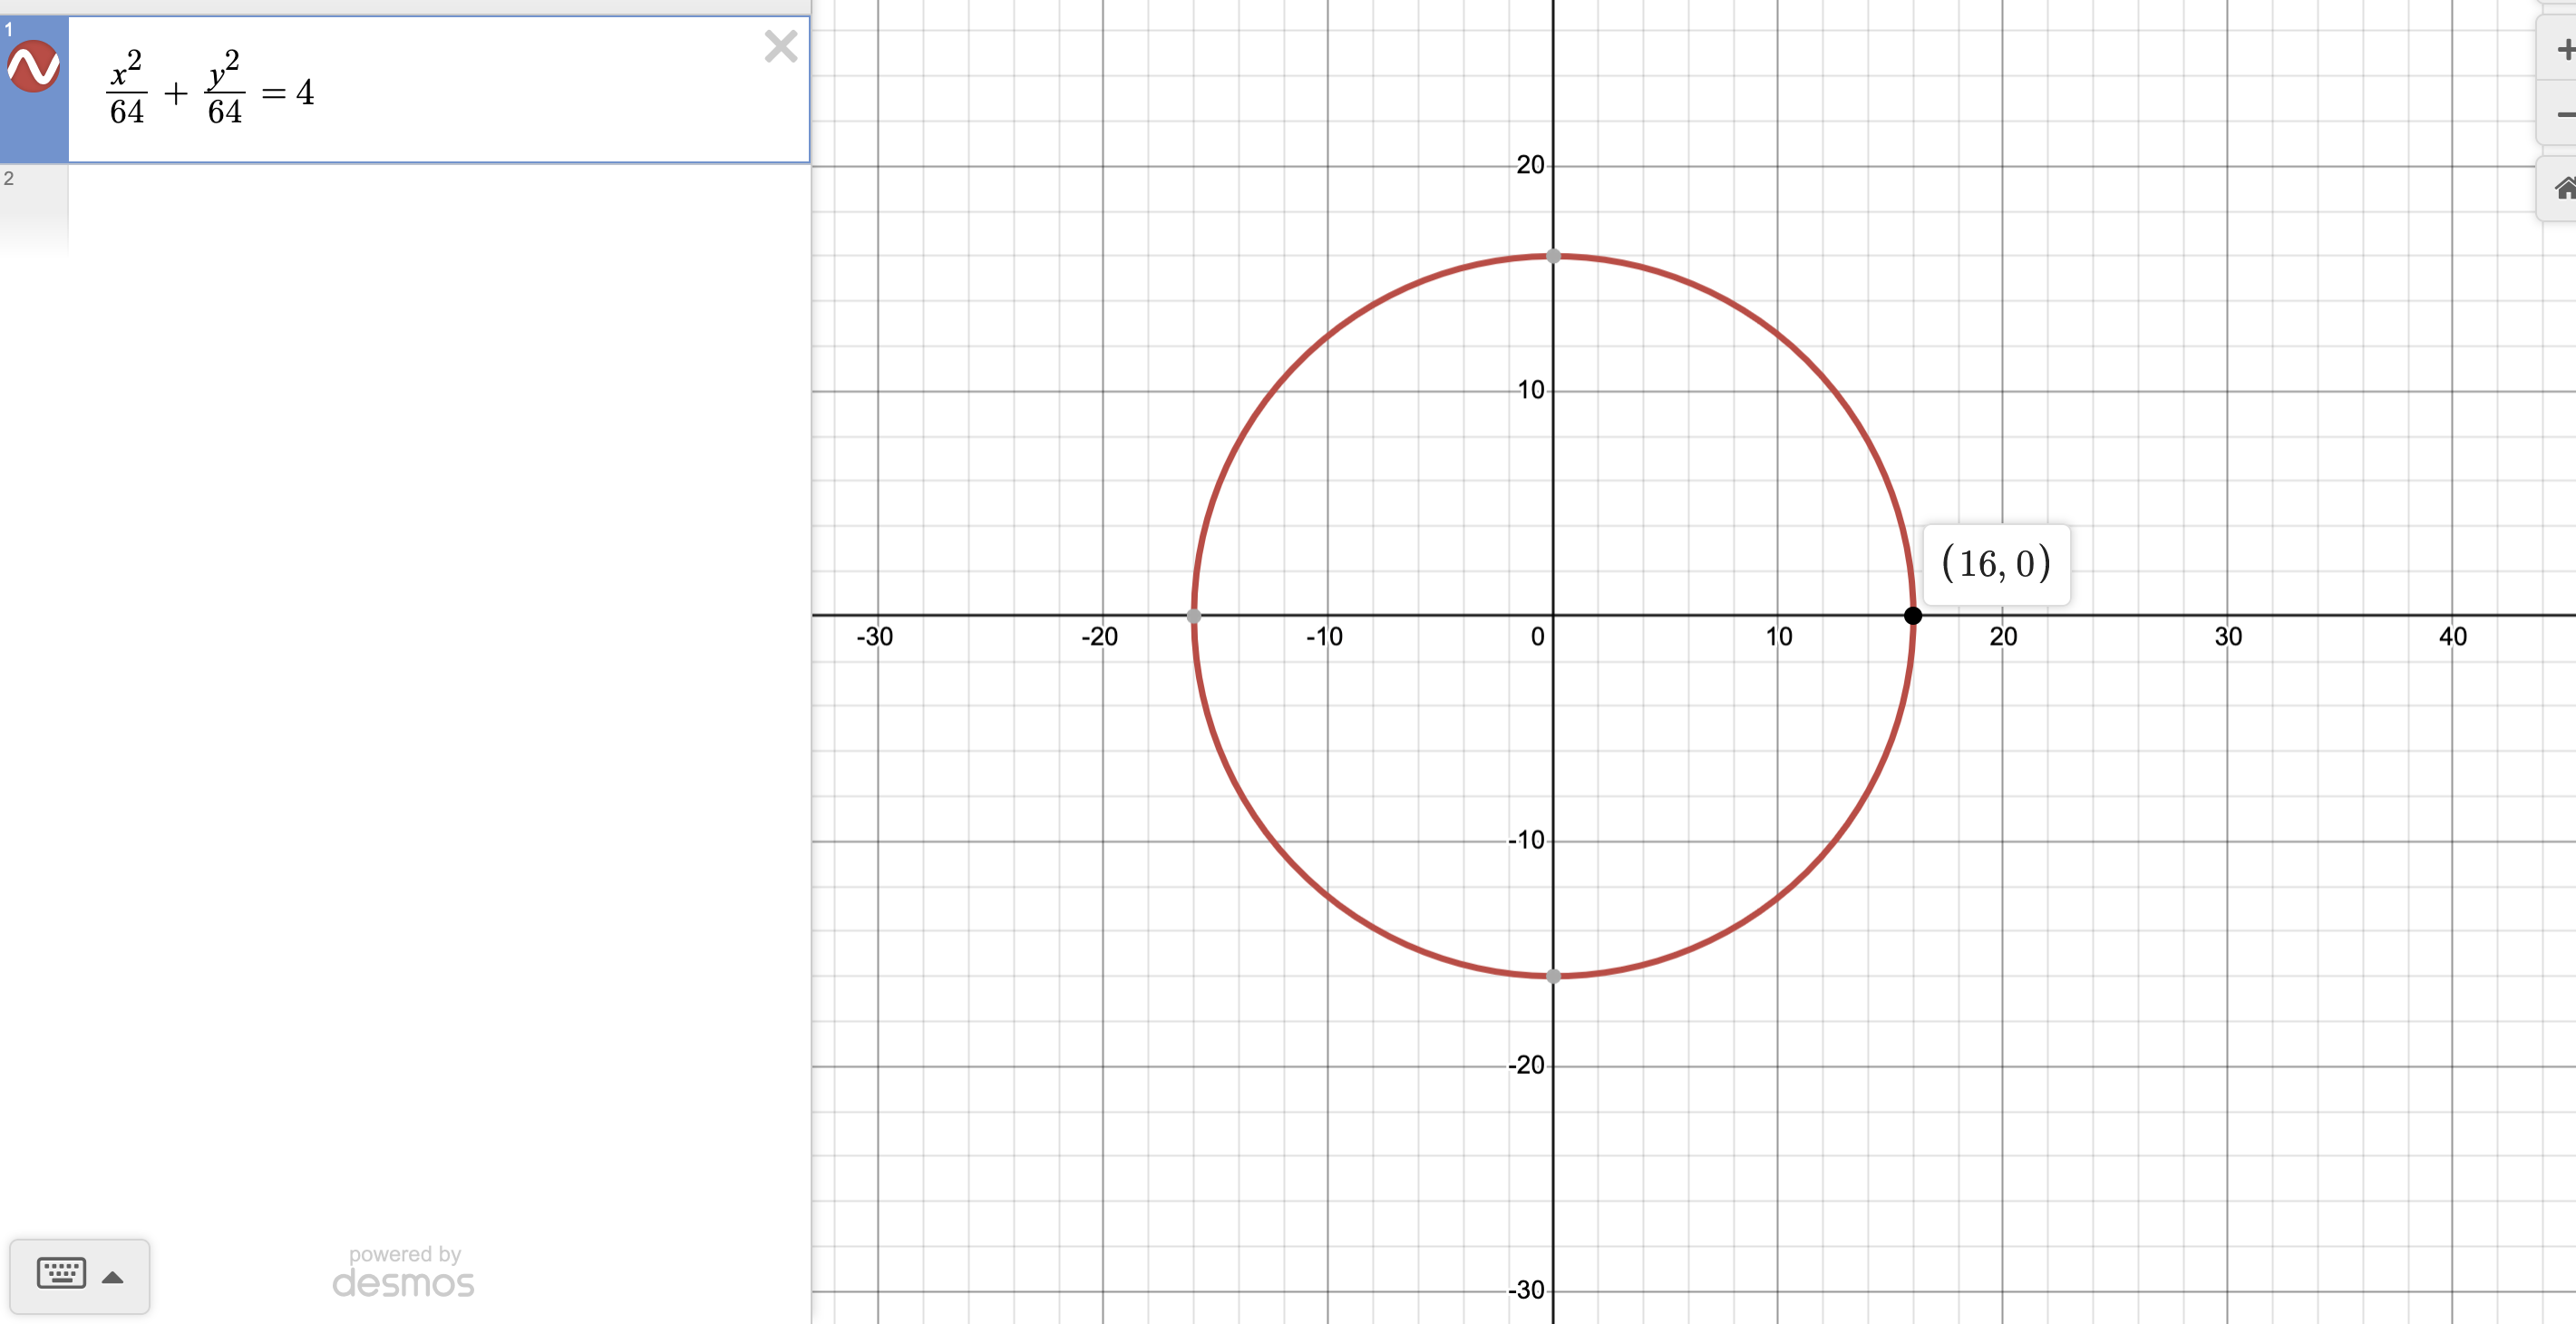
\includegraphics[width = 4in, height = 4in]{43}

\section*{45}
If we change the graph from $\frac{x^2}{9}+\frac{y^2}{25}=1$ to $\frac{x^2}{9}+\frac{y^2}{9}=1$, that is, 
to $x^2+y^2=9$, the graph will no longer be an ellipse, but a circle, namely one with a radius of $3$. If we then change the graph to 
$\frac{x^2}{9}+\frac{y^2}{4}$, the graph will change from the original graph in the following way. In the original graph, $a=3$ and $b=5$. But now, 
$a=3$ and $b=2$. What this means is that the major axis was initially vertical, but now it is horizontal. In addition, the vertices and the co-vertices of the 
first graph were $(0,\pm 5)$ and $(\pm 3,0)$, respectively; but now the vertices and the co-vertices are $(\pm 3,0)$ and $(0,\pm 2)$, respectively: 
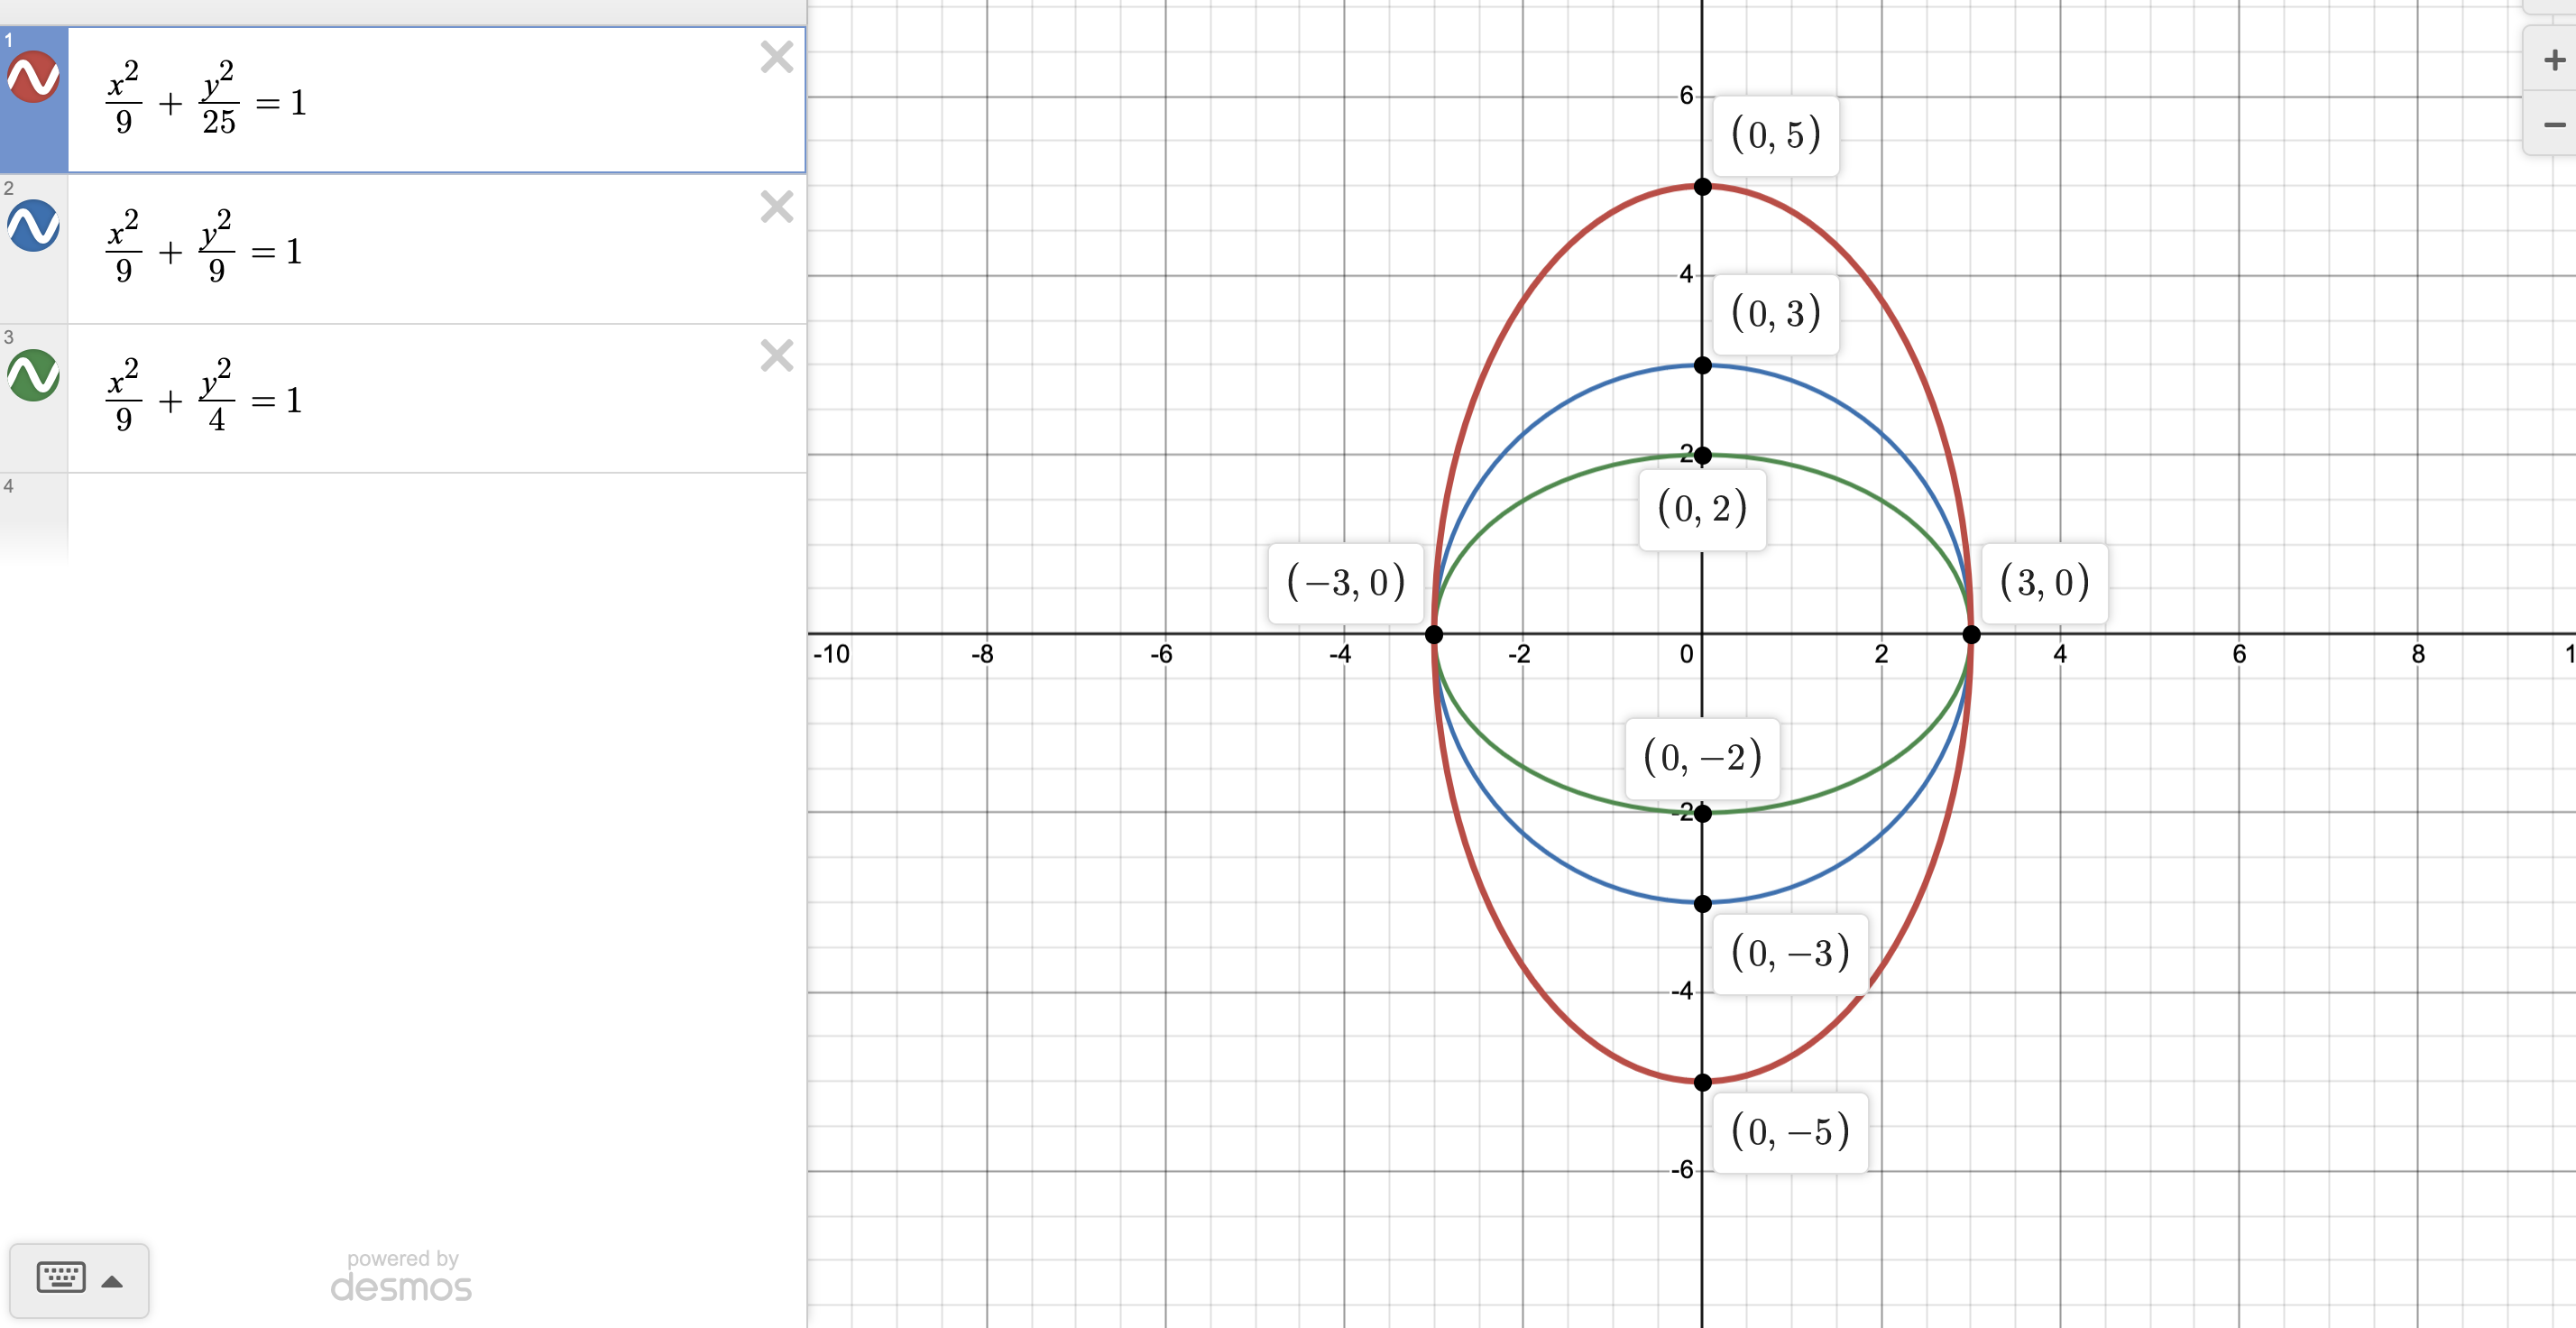
\includegraphics[width = 4in, height = 4in]{45}

\section*{47}
We first consider an ellipse with equation $\frac{x^2}{a^2}+\frac{y^2}{b^2}=1$ with foci at $(c,0)$ and $(-c,0)$. Let us consider the diagram of this ellipse, which 
can be found on page 510. By the definition of an ellipse, we know that the sum of the distances from point $(0,b)$ to $(-c,0)$ and $(c,0)$ is the same as the sum of 
the distances from $(a,0)$ to $(c,0)$ and $(-c,0)$. The distances from $(0,b)$ to $(-c,0)$ and $(c,0)$ are both $\sqrt{b^2+c^2}$, meaning the sum is 
$2\sqrt{b^2+c^2}$. The distance from $(a,0)$ to $(-c,0)$ is $a+c$, and the distance from $(a,0)$ to $(c,0)$ is $a-c$. Thus the sum is 
$a+c+a-c=2a$. Hence:
\[ 2a=2\sqrt{b^2+c^2} \] \[ a=\sqrt{b^2+c^2} \] \[ a^2=b^2+c^2 \] \[ c^2=a^2-b^2 \] which is what we desired to show. Near identical reasoning can be used to prove the result 
in the case of an ellipse with the equation $\frac{x^2}{b^2}+\frac{y^2}{a^2}=1$, except considering the sums of the distances from $(0,a)$ and $(b,0)$ to 
$(0,c)$ and $(-c,0)$. 

\section*{49}
We know that the fied is an ellipse that is between 135 and 185 meters long and between 110 and 155 meters wide. Thus $a$ is between $\frac{135}{2}=67.5$ and 
$\frac{185}{2}=92.5$ meters long and $b$ is between $\frac{110}{2}=55$ and $\frac{155}{2}=77.5$ meters. Thus the equations modeling the largest and smallest fields are 
$\frac{x^2}{92.5^2}+\frac{y^2}{77.5^2}=1$ and $\frac{x^2}{67.5^2}+\frac{y^2}{55^2}=1$, respectively. We know that the area of an ellipse is given by 
$A=\pi ab$. Thus the area of the field is between $\pi 67.5\times 55=3712.5\pi$ and $\pi 92.5\times 77.5=7168.75\pi$, that is, 
$3712\le A\le 7168.75$.

\section*{50}
We are given an ellipse that is $28$ cm long and $16$ cm wide. Thus $a=\frac{28}{2}=14$ and $b=\frac{16}{2}=8$, meaning an equation for the ellipse is (because the major 
axis is horizontal) 
$\frac{x^2}{28^2}+\frac{y^2}{16^2}=1$. We know that \[ c^2=28^2-16^2 \] \[ c=\sqrt{528}=4\sqrt{33} \] meaning the foci are $(\pm 4\sqrt{33},0)$, and thus the distance 
between the foci is $8\sqrt{33}$.

\section*{51}
If I was able to prove the following statement I would have been able to solve this, but I was unable to prove it: The point on the ellipse (with the equation 
$\frac{x^2}{a^2}+\frac{y^2}{b^2}=1$) furthest away from the 
focus $(-c,0)$ is the vertex $(a,0)$, and the point on the ellipse furthest away from the focus $(c,0)$ is $(-a,0)$.

\section*{52}
(a): The reason is as follows. We are given that the plane only has fuel to fly safely 600 miles. We are also given that it is flying from airport $A$ to airport $B$. Thus it 
must be that the sum of the distances from the plane to airport $B$ and airport $A$ is never greater than 600 miles, which is the definition of an ellipse.


(b): We are given that airport $A$ is 450 miles west of airport $B$. Thus the coordinate of airport $A$ is $(-\frac{450}{2},0)=(-225,0)$ and the coordinate of airport $B$ is 
$(\frac{450}{2},0)=(225,0)$.


(c): Suppose the plane flies from airport $A$ straight past airport $B$ to a vertex of the ellipse and then straight back to airport $B$. Thus if flied a total distance of 
$2a$, where $a$ is half the length between the two vertices. Let $d$ be the distance between the focus and the vertex closest to it. When the plane flew past airport $B$ to 
the vertex past it, the sum of the distances from that vertex to the two foci was $450+b+b=450+2b$. Thus \[ 450+2b=600 \] \[ b=75 \] What this means is that the vertices are 
$(225+75=300,0)$ and $(-225-75=-300,0)$, that is, $(\pm 300,0)$.


(d): We know $a$ and the foci ($\pm 225,0$):
\[ b^2=300^2-225^2 \] \[ b=\sqrt{39375} \] meaning an equation for the ellipse is \[ \frac{x^2}{300^2}+\frac{y^2}{(\sqrt{39375})^2}=1 \]
\[ \frac{x^2}{300^2}+\frac{y^2}{39375}=1 \]

\section*{53}
From the given diagram, we can form three right triangles. One is in the top left corner. It has one unknown side $A$, and a hypotenuse of $2$, and a third 
side of $x$. Thus $A^2=2^2-x^2$. The second triangle is the second largest triangle of the diagram. It has one unkown side $B$, a hypotenuse of $6$, and a third side of 
$y$. Thus $B^2=6^2-y^2$. The third triangle is the largest triangle in the diagram. It has a known hypotenuse of 8, and two unknown sides: $A+y$ and 
$B+x$. Thus, we have the following:
\[ 8^2=(A+y)^2+(B+x)^2 \]
\[ 64=A^2+2Ay+y^2+B^2+2Bx+x^2 \]
\[ 64=(4-x^2)+2(\sqrt{4-x^2})y+y^2+(36-y^2)+2(\sqrt{36-y^2})x+x^2 \]
\[ 24=2(\sqrt{4-x^2}y+\sqrt{36-y^2}x) \]
\[ 12=\sqrt{4-x^2}y+\sqrt{36-y^2}x \]
\[ 12-\sqrt{4-x^2}y=\sqrt{36-y^2}x \]
\[ 144+(4-x^2)y^2-24\sqrt{4-x^2}y=(36-y^2)x^2 \]
\[ 144+4y^2-x^2y^2-36x^2+x^2y^2=24\sqrt{4-x^2}y \]
\[ 144+4y^2-36x^2=24\sqrt{4-x^2}y \]
\[ 36+y^2-9x^2=6\sqrt{4-x^2}y \]
\[ 36(36+y^2-9x^2)+y^2(36+y^2-9x^2)-9x^2(36+y^2-9x^2)=36y^2(4-x^2) \]
\[ 1296+36y^2-324x^2+36y^2+y^4-9x^2y^2-324x^2-9x^2y^2+81x^4=144y^2-36x^2y^2 \]
\[ 1296+72y^2-648x^2-18x^2y^2+81x^4+y^4=144y^2-36x^2y^2 \]
\[ 81x^4+y^4+18x^2y^2-648x^2-72y^2+1296=0 \]

\end{document}
